\documentclass[12pt,draft]{Manuscript}

\usepackage[page,title,toc]{appendix}
\usepackage{amsfonts}
\usepackage{amsmath}
\usepackage{array}
\usepackage{booktabs}
\usepackage{chngcntr}
\usepackage{cleveref}
\usepackage{epigraph}
\usepackage{etoolbox}
\usepackage{framed}
\usepackage{listings}
\usepackage{longtable}
\usepackage{multirow}
\usepackage{rotating}
\usepackage{subfig}
\usepackage{textcase}
\usepackage{textcomp,upquote}
\usepackage{xcolor}

\counterwithout{footnote}{chapter}


\usepackage{times}
\usepackage{amssymb,amsmath}
\usepackage{ifxetex,ifluatex}
\usepackage{fixltx2e} % provides \textsubscript
\ifnum 0\ifxetex 1\fi\ifluatex 1\fi=0 % if pdftex
  \usepackage[T1]{fontenc}
  \usepackage[utf8]{inputenc}
\else % if luatex or xelatex
  \ifxetex
    \usepackage{mathspec}
    \usepackage{xltxtra,xunicode}
  \else
    \usepackage{fontspec}
  \fi
  \defaultfontfeatures{Mapping=tex-text,Scale=MatchLowercase}
  \newcommand{\euro}{€}
\fi
\usepackage{natbib}
\usepackage{listings}
\usepackage{graphicx}
\makeatletter
\def\maxwidth{\ifdim\Gin@nat@width>\linewidth\linewidth\else\Gin@nat@width\fi}
\def\maxheight{\ifdim\Gin@nat@height>\textheight\textheight\else\Gin@nat@height\fi}
\makeatother
% Scale images if necessary, so that they will not overflow the page
% margins by default, and it is still possible to overwrite the defaults
% using explicit options in \includegraphics[width, height, ...]{}
\setkeys{Gin}{width=\maxwidth,height=\maxheight,keepaspectratio}
\ifxetex
  \usepackage[setpagesize=false, % page size defined by xetex
              unicode=false, % unicode breaks when used with xetex
              xetex]{hyperref}
\else
  \usepackage{hyperref}
\fi
\hypersetup{breaklinks=true,
            bookmarks=true,
            pdfauthor={Christopher Scott Corley},
            pdftitle={Online Topic Modeling for Software Maintenance},
            colorlinks=true,
            citecolor=brown,
            urlcolor=blue,
            linkcolor=magenta,
            pdfborder={0 0 0}}
% Make links footnotes instead of hotlinks:
\renewcommand{\href}[2]{#2\footnote{\url{#1}}}

\title{Online Topic Modeling for Software Maintenance}
\author{Christopher Scott Corley}
\date{2014}
\location{\MakeUppercase{Tuscaloosa, Alabama}}
\thesistype{\MakeUppercase{A dissertation (proposal)}}
\submissioninfo{
Submitted in partial fulfillment of the requirements\\
for the degree of Doctor of Philosophy\\
in the Department of Computer Science\\
in the Graduate School of\\
The University of Alabama\\
}
\setlength\epigraphwidth{\textwidth}
\setlength\epigraphrule{0pt}

\definecolor{lightred}{RGB}{175,50,50}
\definecolor{lightgreen}{RGB}{0,150,0}
\definecolor{lightblue}{RGB}{50,50,175}

\lstdefinelanguage{diff}{
  morecomment=[f][\color{lightblue}]{diff },
  morecomment=[f][\color{lightblue}]{index },
  morecomment=[f][\color{lightblue}]{@@},     % group identifier
  morecomment=[f][\color{lightred}]-,         % deleted lines
  morecomment=[f][\color{lightgreen}]+,       % added lines
  morecomment=[f][\color{lightblue}]{---}, % Diff header lines (must appear after +,-)
  morecomment=[f][\color{lightblue}]{+++},
}
\hyphenation{}

\newcommand{\attn}[1]{{\color{red}#1}}
\newcommand{\desc}[1]{{\emph{\color{blue}#1}}}
\newcommand{\needcite}{\attn{\tiny{[cite]}}}

\newcommand{\committeemembers}{
\MakeUppercase{Jeffrey C. Carver, Committee Chair}\\
\MakeUppercase{Nicholas A. Kraft}\\
\MakeUppercase{Jeffrey G. Gray}\\
}

\begin{document}
\maketitle

\begin{abstract}
    I can write an abstract.
    
    It might be long.
\end{abstract}

{
\hypersetup{linkcolor=black}
\setcounter{tocdepth}{2}
\tableofcontents
}
\begin{abbreviations}
    \begin{center}
\begin{longtable}{l    l}
TEST & TEST
\end{longtable}
\end{center}

\end{abbreviations}
\listoftables
\listoffigures

\clearpage
\begin{body}
\chapter{Introduction}\label{introduction}

Basic idea:

\begin{itemize}
\itemsep1pt\parskip0pt\parsep0pt
\item
  Lots of software maintenance tasks being automated by topic modeling
\item
  Topic modeling is now online, but we are not using it?
\item
  We build topic models from source code, meaning the model is tied to a
  specific instance of it

  \begin{itemize}
  \itemsep1pt\parskip0pt\parsep0pt
  \item
    This makes the models not very useful in practice. Slow, outdated.
  \end{itemize}
\item
  Why not build topic models out of the changesets

  \begin{itemize}
  \itemsep1pt\parskip0pt\parsep0pt
  \item
    Changesets are a view of the source code over time
  \item
    We can build comparable topic models with changesets
  \end{itemize}
\item
  We can better evaluate the accuracy of the techniques because we can
  process changesets overtime, sort of like a similuation of what
  actually happened (or as close as we can get to it)
\item
  We only need \emph{one} model per branch. The doc-topic can be any
  \emph{any} granularity desired, and the model does not need to be
  re-built from scratch everytime.
\item
  Look at how does the changeset model compare to the typical source
  code model

  \begin{itemize}
  \itemsep1pt\parskip0pt\parsep0pt
  \item
    Combinations of: context/added/removed lines in the diff
  \item
    Per-file changed or whole changeset
  \item
    Ignore whitespaces
  \item
    Only look at the changed words instead of the entire lines

    \begin{itemize}
    \itemsep1pt\parskip0pt\parsep0pt
    \item
      Combinations of: context/added/removed
    \end{itemize}
  \end{itemize}
\end{itemize}

Software developers are often confronted with maintenance tasks that
involve navigation of repositories that preserve vast amounts of project
history. Navigating these software repositories can be a time-consuming
task, because their organization can be difficult to understand.
Fortunately, topic models such as latent Dirichlet allocation (LDA)
\citep{Blei-etal:2003} can help developers to navigate and understand
software repositories by discovering topics (word distributions) that
reveal the thematic structure of the data
\citep{Linstead-etal:2007, Thomas-etal:2011, Hindle-etal:2012}.

Program comprehension is a prerequisite to incremental change. A
software developer who is tasked with changing a large software system
spends effort on program comprehension activities to gain the knowledge
needed to make the change \citep{Corbi:1989}. For example, the developer
spends effort to understand the system architecture or to locate the
parts of the source code that implement the feature(s) being changed.
Gaining such knowledge can be a time-consuming task, especially for
developers who are unfamiliar with the system. Topic models of source
code can help such developers to understand the system by revealing a
latent structure that is not obvious from the package hierarchy or
system documentation \citep{Savage-etal:2010}.

Topic models are clusters of source code entities (e.g., classes) that
are grouped by their natural language content (i.e., the words in their
identifiers, comments, and literals). Such topics often correspond to
the concepts and features implemented by the source code
\citep{Baldi-etal:2008}, and exploring such topics shows promise in
helping developers to understand the entities that make up a system and
to understand how those entities relate
\citep{Kuhn-etal:2007, Maskeri-etal:2008, Savage-etal:2010, Gethers-etal:2011a}.
Recent approaches to exploring linguistic topics in source code use
machine learning techniques that model correlations among words, such as
latent semantic indexing (LSI) \citep{Deerwester-etal:1990} and latent
Dirichlet allocation (LDA) \citep{Blei-etal:2003}, and ML techniques
that also model correlations among documents, such as RTM
\citep{Chang-Blei:2010}.

Topic models of source code have many applications in addition to
general program comprehension. These applications include feature
location\needcite, bug localization \citep{Rao-etal:2013}, triaging
incoming change requests \citep{Kagdi-etal:2012}, aspect mining
\citep{Baldi-etal:2008}, and traceability link recovery
\citep{Asuncion-etal:2010}. Yet, while researchers have had success in
using topic models on source code entities, there is a fundamental issue
with the current approaches. This issue is that the input documents used
to build a topic model are source code entities, and will be the
motivating point of this work.

\section{Motivation}\label{motivation}

When modeling a source code repository, the corpus typically represents
a snapshot of the code. That is, a topic model is often trained on a
corpus that contains documents that represent files from a particular
version of the software. Keeping such a model up-to-date is expensive,
because the frequency and scope of source code changes necessitate
retraining the model on the updated corpus. However, it may be possible
to automate certain maintenance tasks without a model of the complete
source code. For example, when assigning a developer to a change task, a
topic model can be used to associate developers with topics that
characterize their previous changes. In this scenario, a model of the
changesets created by each developer may be more useful than a model of
the files changed by each developer. Moreover, as a typical changeset is
smaller than a typical file, a changeset-based model is less expensive
to keep current than a file-based model.

While using file-based models is a natural fit for program comprehension
tasks such as feature location and bug localization, they still are
unable to stay up-to-date entirely. Additionally, much of the work for
assigning developers to change requests still uses files as input and an
array of heuristics to identify a developer
\citep{Kagdi-etal:2012}\needcite. These methods also have the same flaw
in that they ultimately rely on files for information.

Like Rao et al. \citep{Rao-etal:2013}, the motivation of this work is to
create topic models that can be incrementally updated over time.
However, unlike Rao et al., we can rely on the source code history
itself to build the model without needing to manually adjust model
latent variables. This gains the benefit of an increase in query time,
but also could lead to a more reliable model.

\section{Research Goals, Questions, and
Hypotheses}\label{research-goals-questions-and-hypotheses}

The primary research goal of this proposal is to evaluate the
performance and reliability of topic models built on the source code
histories. This will require configuring and executing studies in
various contexts of software maintenance work, such as feature location,
bug localization, and developer identification.

A secondary goal is to create a practical framework for building models
that can be used in multiple contexts. This will require building a
prototype tool that could be used by both researchers and practitioners.

\section{Limitations and Assumptions}\label{limitations-and-assumptions}

\chapter{Related work}\label{related-work}

In this section, we review the literature in detail. First, we review
various text retrieval models. We then discuss how these TR approaches
are applied in software engineering. Finally, we discuss various areas
of software engineering in which TR has been applied.

\section{Text Retrieval}\label{related-general-TR}

In this section, we review and summarize the terminology and text
retrieval process.

\subsection{Terminology}\label{terminology}

We use the following terminology to describe text retrieval:

\begin{description}
\itemsep1pt\parskip0pt\parsep0pt
\item[term (word), \(w\):]
the smallest free-form of a language
\item[token:]
a sequence of non-whitespace characters containing one or more term
\item[document, \(d\):]
a sequence of \(D\) terms \(w_1, w_2, ..., w_D\), often represented as a
bag of words (i.e., \(M\)-length vector of term frequencies or weights)
\item[corpus, \(C\):]
a sequence of \(N\) documents \(d_1, d_2, ..., d_N\) (i.e., a
\(M \times N\) document-term matrix)
\item[vocabulary, \(V\):]
a set of \(M\) unique terms that appear in a corpus
\(\{w_1, w_2, ..., w_M\}\)
\item[topic, \(z\):]
a concept or theme of related terms, often represented as a distribution
of term proportions
\item[topic model, \(\phi\):]
a mathematical representation of the thematic structure of a corpus, or
how much a term \(w\) contributes to each topic \(z\) (i.e., a
\(M \times K\) topic-term matrix)
\item[inferrence, \(\theta_d\)]
the thematic structure of a given document (i.e., a \(K\)-length topic
proportion vector)
\item[index, \(\theta\):]
a corpus that has been transformed for searching, e.g., in LDA by
inferring the thematic structure of each document (i.e., a
\(N \times K\) document-topic matrix)
\item[query, \(q\):]
a document created by a user
\item[search engine:]
ranks documents by their similarity to a query
\end{description}

\subsection{Text Retrieval Process}\label{text-retrieval-process}

The text retrieval process consists of two general steps: document
extraction and retrieval.

\begin{figure}[htbp]
\centering
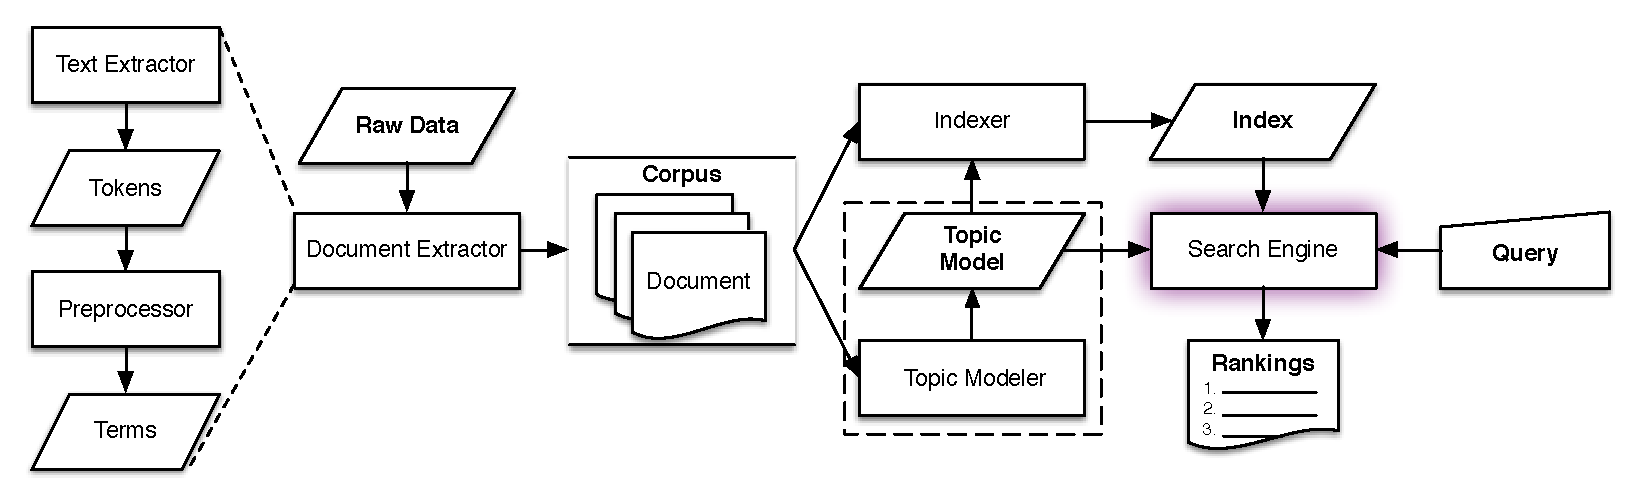
\includegraphics{figures/text-retrieval.pdf}
\caption{The general text retrieval process\label{fig:TR}}
\end{figure}

\subsubsection{Document extraction}\label{document-extraction}

The left side of Figure \ref{fig:TR} illustrates the document extraction
process. A document extractor takes raw data (e.g., text files) and
produces a corpus as output. Each document in the corpus contains the
words associated to the origin (e.g., a file). The text extractor is the
first part of the document extractor. It produces a token stream for
each document in the data.

The preprocessor is the second part of the document extractor. It
applies a series of transformations to each token and produces one or
more terms from the token. The transformations commonly used are:

\begin{enumerate}
\def\labelenumi{\arabic{enumi}.}
\item
  \begin{description}
  \itemsep1pt\parskip0pt\parsep0pt
  \item[Split:]
  separate tokens into constituent words by non-alphabetical characters
  or convention (e.g., ``two-thirds'' becomes ``two'' and ``thirds'')
  \end{description}
\item
  \begin{description}
  \itemsep1pt\parskip0pt\parsep0pt
  \item[Normalize:]
  replace each upper case letter with the corresponding lower case
  letter, or vice versa
  \end{description}
\item
  \begin{description}
  \itemsep1pt\parskip0pt\parsep0pt
  \item[Filter:]
  remove common words such as natural language articles (e.g., ``an'' or
  ``the''), stop words, or short words
  \end{description}
\item
  \begin{description}
  \itemsep1pt\parskip0pt\parsep0pt
  \item[Stem:]
  remove prefixes and suffixes to leave just the root word (e.g.,
  ``name'', ``names'', ``named'', and ``naming'' all reduce to
  ``name''). A common stemmer used is by \citet{Porter:1980}.
  \end{description}
\item
  \begin{description}
  \itemsep1pt\parskip0pt\parsep0pt
  \item[Weigh:]
  adjust the representation of a term in a document by some scheme, such
  as term-frequency inverse-document-frequency (tf-idf)
  \citep{Salton-Buckley:1988}
  \end{description}
\item
  \begin{description}
  \itemsep1pt\parskip0pt\parsep0pt
  \item[Prune:]
  remove term that occur in, for example, over 80\% or under 2\% of the
  documents \citep{Madsen-etal:2004}.
  \end{description}
\end{enumerate}

\subsubsection{Model Construction and
Retrieval}\label{model-construction-and-retrieval}

The right side of Figure \ref{fig:TR} illustrates the retrieval process.
The main component of the retrieval process is the search engine, which
must first be constructed. A search engine typically consists of a
model, an index, and a classifier for ranking.

The primary function of the search engine is to rank documents in
relation to the query. First, the corpus is transformed into an index.
Next, the engine takes a pairwise classification of the query to each
document in the index and ranks the documents according to similarity. A
similarity measure for probability distributions, such as cosine
similarity or Hellinger distance, can be used for these pairwise
comparisons. Hellinger distance (\(H\)) can be defined as:

\begin{equation}
    H(P, Q) = \frac{1}{\sqrt{2}} \; \sqrt{\sum_{i=1}^{K} (\sqrt{P_i} - \sqrt{Q_i})^2}
\label{eq:hellinger}
\end{equation}

where \(P\) and \(Q\) are two discrete probability distributions of
length \(K\).

\section{Text Retrieval for Software}\label{related-software-TR}

\subsection{Terminology}\label{terminology-1}

We adopt and extend terminology from \citet{Biggers-etal:2014}. In
particular, we define the following:

\begin{description}
\itemsep1pt\parskip0pt\parsep0pt
\item[entity]
a named source element such as a method, class, or package
\item[identifier]
a token representing the name of an entity
\item[comment]
a sequence of tokens delimited by language specific markers (e.g.,
\lstinline!/* */! or \lstinline!#!)
\item[literal]
a sequence of tokens delimited by language specific markers (e.g.,
\lstinline!' '! for strings)
\end{description}

In addition to the transformations outlined in Section
\ref{document-extraction}, extended transformations
\citep{Marcus-etal:2004, Marcus-Menzies:2010} commonly used in software
are:

\begin{enumerate}
\def\labelenumi{\arabic{enumi}.}
\item
  \begin{description}
  \itemsep1pt\parskip0pt\parsep0pt
  \item[Split:]
  separate tokens into constituent words based on common coding style
  conventions (e.g., the use of camel case or underscores) and on the
  presence of non-letters (e.g., punctuation or digits)
  \end{description}
\item
  \begin{description}
  \itemsep1pt\parskip0pt\parsep0pt
  \item[Filter:]
  remove common words such programming language keywords, or standard
  library entity names
  \end{description}
\item
  \begin{description}
  \itemsep1pt\parskip0pt\parsep0pt
  \item[Weight:]
  adjust the representation of a term in a document by some scheme, such
  as by the entity type \citep{Bassett-Kraft:2013}.
  \end{description}
\end{enumerate}

\subsection{Boolean Model}\label{boolean-model}

The Boolean model is the simplest of the models used for constructing a
search engine. This approach builds an index of the corpus by treating
each document as a set of unique terms. Essentially, all terms are
weighted equally: either the term is in the document or it isn't.
Queries can be constructed with single keywords joined by boolean
expressions such as \lstinline!AND!, \lstinline!OR!, and
\lstinline!NOT!.

\subsection{Vector Space Model}\label{vector-space-model}

The Vector Space Model (VSM) is an algebraic model introduced by
\citet{Salton-etal:1975}. VSM uses the corpus directly as an index. Each
document in the index is represented as a vector of term weights: words
which appear in a document will be assigned a weight by some weighting
scheme, and words that do not appear have weights of zero. Queries are
transformed into a vector of term weights of the same length.

\subsection{Topic Models}\label{topic-models}

\subsubsection{Latent Semantic Indexing}\label{latent-semantic-indexing}

Latent semantic indexing \citep{Deerwester-etal:1990} is an indexing and
retrieval methodology that extends the VSM.

\citet{Rehurek:2011} outlines extensions to LSI which enable the
algorithm to be \emph{online}. Online LSI allows the model to be updated
incrementally without needing to know about the documents prior to model
construction.

\subsubsection{Latent Dirichlet
Allocation}\label{latent-dirichlet-allocation}

Latent Dirichlet allocation \citep{Blei-etal:2003} is a generative topic
model. LDA models each document in a corpus of discrete data as a finite
mixture over a set of topics and models each topic as an infinite
mixture over a set of topic probabilities. That is, LDA models each
document as a probability distribution indicating the likelihood that it
expresses each topic and models each topic that it infers as a
probability distribution indicating the likelihood of a word from the
corpus being assigned to the topic.

\citet{Hoffman-etal:2010} introduce a version of LDA which is online.
\citet{Zhai-Boyd-Graber:2013} introduce an extension of LDA in which the
model also does not need to know about the corpus vocabulary prior to
training.

\section{Feature location}\label{related-flt}

\section{Developer identification}\label{related-triage}

\section{Configuration of Topic Models}\label{related-config}

\chapter{Previous Work}\label{previous-work}

\section{Traceability link recovery}\label{tefse2011}

\section{Modeling ownership}\label{icpc2012}

\section{Duplicate bug report detection}\label{msr2013}

\section{Modeling changeset topics}\label{mud2014}

This section discusses the work in \citet{Corley-etal:2014}.

\subsection{Terminology}\label{terminology-2}

In addition to the terminology described in Section \ref{terminology},
we use the following terminology to describe document extraction of
changesets.

\begin{description}
\itemsep1pt\parskip0pt\parsep0pt
\item[diff:]
set of text which represents the differences between two texts
\item[patch:]
a set of instructions (i.e., diffs) that is used to transform one set of
texts into another
\item[context lines:]
lines of a diff that denote text useful for transforming the text, but
do not represent the differences
\item[added lines:]
lines of a diff that were \emph{added} in order to transform the first
text into the second
\item[removed lines:]
lines of a diff that were \emph{removed} in order to transform the first
text into the second
\item[changeset]
ideally represents a single feature modification, addition, or deletion,
which may crosscut many source code entities
\item[commit]
a representation of a changeset in a version control system, such as Git
or Subversion.
\end{description}

\subsection{Approach}\label{approach}

\begin{itemize}
\itemsep1pt\parskip0pt\parsep0pt
\item
  Document extraction
\item
  Preprocessing
\item
  Training
\item
  Retrieval
\end{itemize}

\begin{figure*}[t]
\centering
\begin{lstlisting}[language=diff, basicstyle=\ttfamily]
diff --git a/lao b/tzu
index 635ef2c..5af88a8 100644
--- a/lao
+++ b/tzu
@@ -1,7 +1,6 @@
-The Way that can be told of is not the eternal Way;
-The name that can be named is not the eternal name.
 The Nameless is the origin of Heaven and Earth;
-The Named is the mother of all things.
+The named is the mother of all things.
+
 Therefore let there always be non-being,
   so we may see their subtlety,
 And let there always be being,
@@ -9,3 +8,6 @@ And let there always be being,
 The two are the same,
 But after they are produced,
   they have different names.
+They both may be called deep and profound.
+Deeper and more profound,
+The door of all subtleties!
\end{lstlisting}
\caption{Example of a \texttt{git diff}}
Black or blue lines denote metadata about the change useful for patching.
In particular, black lines represent context lines (beginning with a single space).
Red lines (beginning with a single~\texttt{-}) denote line removals,
and green lines (beginning with a single~\texttt{+}) denote line additions.
\label{fig:diff}
\vspace{-10pt}
\end{figure*}

\chapter{Proposed work}\label{proposed-work}

In this chapter, I outline the proposed work and methodologies to be
used for each.

\section{Feature location}\label{study-flt}

Feature location is a program comprehension activity in which a
developer inspects source code to locate the classes or methods that
implement a feature of interest.

\subsection{Motivation}\label{motivation-1}

Many feature location techniques (FLTs) are based on text retrieval
models, and in such FLTs it is typical for the models to be built from
source code snapshots. However, source code evolution leads to model
obsolescence and thus to the need to retrain the model from the latest
snapshot.

\subsection{Background}\label{flt-background}

\begin{figure}[htbp]
\centering
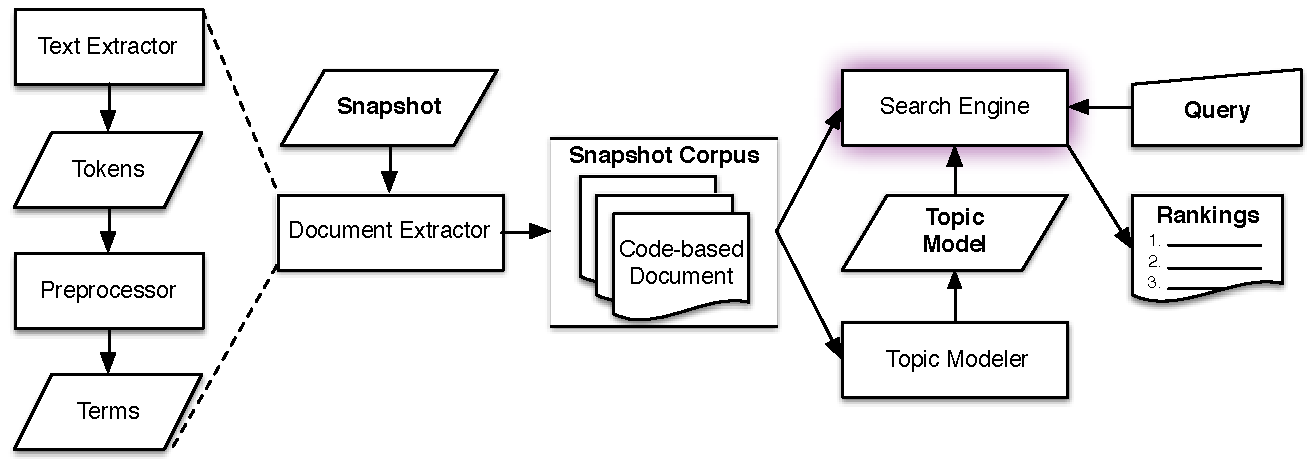
\includegraphics{figures/snapshot-flt.pdf}
\caption{Typical feature location process\label{fig:snapshot-flt}}
\end{figure}

The left side of Figure \ref{fig:snapshot-flt} illustrates the document
extraction process. A document extractor takes source code as input and
produces a corpus as output. Each document in the corpus contains the
words associated with a source code entity such as a class or method.
The text extractor is the first part of the document extractor. It
parses the source code and produces a token stream for each class. The
preprocessor is the second part of the document extractor. It applies a
series of transformations to each token and produces one or more words
from the token.

The right side of Figure \ref{fig:snapshot-flt} illustrates the
retrieval process. The main prerequisite of the retrieval process is to
build the search engine. The search engine is constructed from the topic
model trained from the corpus and an index of that corpus inferred from
that model, known as \(\theta\). The primary function of the search
engine is to rank documents in relation to the query. The search engine
performs a pairwise classification of the query to each document and
ranks the documents according score.

To accomplish the classification step using a topic model, the search
engine infers \(\theta_{Snapshot}\), i.e., the topic-document
probability distribution of each document in the snapshot corpus, as
well as \(\theta_{Query}\), i.e., the topic-document probability
distribution of the query. Then a similarity measure for probability
distributions, such as cosine similarity or Hellinger distance, can be
used to make pairwise comparisons between \(\theta_{Query}\) and
\(\theta_{Snapshot}\).

\subsection{Proposal}\label{proposal}

In this proposal, we introduce a topic-modeling-based FLT in which the
model is built incrementally from source code \emph{changesets}. By
training an online learning algorithm using changesets, the FLT
maintains an up-to-date model without incurring the non-trivial
computational cost associated with retraining traditional FLTs.

\subsubsection{Approach}\label{flt-proposed-approach}

\begin{figure}[htbp]
\centering
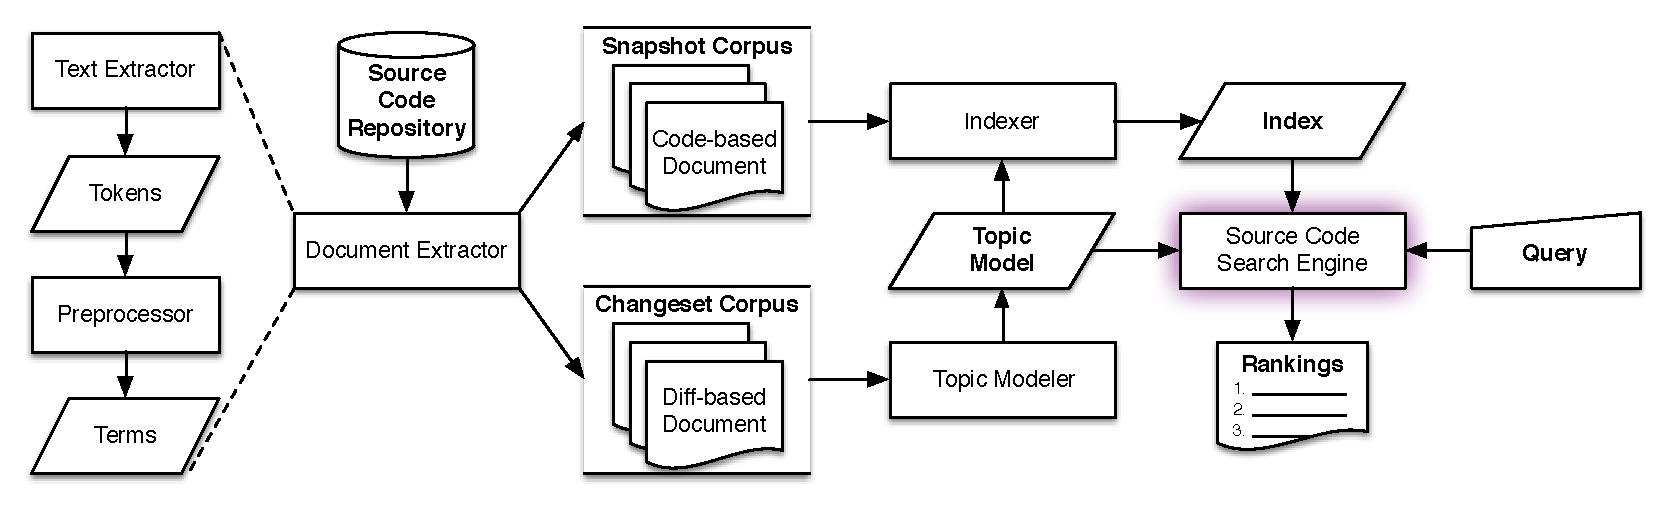
\includegraphics{figures/changeset-flt.pdf}
\caption{Feature location using changesets\label{fig:changeset-flt}}
\end{figure}

The changeset topic modeling approach requires two types of document
extraction: one for the snapshot of the state of source code at a commit
of interest, such as a tagged release, and one for the every changeset
in the source code history leading up to that commit. The left side of
Figure \ref{fig:changeset-flt} illustrates the dual-document extraction
approach.

The document extraction process for the snapshot remains the same as
covered in Section \ref{flt-background}. The document extractor for the
changesets parses each changeset for the removed, added, and context
lines. From there, each line is tokenized by the text extractor. In a
changeset it may be desirable to parse further for source code entities
using island grammar parsing \citep{Moonen:2001}, although not necessary
for this approach. It may also be desirable to only use portions of the
changeset, such as only using added or removed lines. The same
preprocessor transformations as before also occur in changesets.

The right side of Figure \ref{fig:changeset-flt} illustrates the
retrieval process. The key intuition to our approach is that a topic
model such as LDA or LSI can infer any given document's topic
proportions regardless of the documents used to train the model. Hence,
we train a topic model on the changeset corpus, but search for related
documents over the snapshot corpus. In the search engine, we can use a
dynamic programming to keep \(\theta_{Snapshot}\) up-to-date as new
changesets are added to the model. That is, upon a update to the model,
new inferences of only the source code documents affected by this
changeset are made. Additionally, we can then query the model as needed
and rank the results of that query against \(\theta_{Snapshot}\). Note
that we never infer a \(\theta_{Changeset}\) for the changeset documents
on which the model is built.

To leverage the online functionality of the topic models, we can also
intermix the model training and retrieval steps. First, we initialize a
model in online mode. Then, as changes are made, the model is updated
with the new changesets as they are committed. That is, with changesets,
we incrementally update a model and can query it at any moment. This
insight means that we can also evaluate our approach \emph{temporally}.
That is, we we can approximate how the FLT would perform throughout the
evolution of a project.

\subsubsection{Evaluation}\label{evaluation}

\begin{itemize}
\itemsep1pt\parskip0pt\parsep0pt
\item
  FLT using both LSI and LDA
\item
  \citet{Dit-etal:2013}
\item
  \citet{Moreno-etal:2014}
\item
  These datasets contain \textgreater{}1200 defects and features from 14
  OSS Java projects
\item
  We can also do temporal stuff to approximate how the FLT would perform
  throughout the evolution of a project.
\end{itemize}

\section{Developer identification}\label{study-triage}

\subsection{Motivation}\label{motivation-2}

Software features are functionalities that are defined by requirements
and are accessible to developers and users. Software change is
continual, because new features must be added to meet revised
requirements, existing features must be enhanced to satisfy increased
expectations, and defective features (i.e., bugs) must be removed to
achieve intended behavior. Changes to a software system are proposed by
developers or users, who submit change requests to the project issue
tracker. Change requests are sometimes called issue reports, and
specific kinds of change requests include feature requests, enhancement
requests, and bug reports.

Triaging a change request involves several steps that can be completed
either by a single person or by a team of developers in a triage
meeting. How triage occurs differs from team to team, but the general
steps required are as follows. First, the triager(s) must see if the
request has enough information to be considered. It is marked as a
duplicate if the request already exists. After it is confirmed that the
request is new and has enough information, a decision must be made if
and how soon it will be completed based on its severity, frequency,
risk, and other factors. Finally, the triager assigns a request to the
developer. Ultimately, the goal of triage is deciding priority of the
request and assignment to the developer that is best suited to complete
the change request.

Triaging is a common and difficult task. Triage is even more difficult
on projects where developer teams are large or geographically
distributed \citep{Herbsleb-etal:2001}. A project member triaging a
change request will need to consider several factors in order to
correctly assign the change request to a set of developers with
appropriate expertise \citep{McDonald-Ackerman:1998}. Triaging requires
contextual knowledge about the product, team structure, individual
expertise, workload balance, and development schedules in order to
correctly assign a change request.

Triaging can be a time consuming and error prone process when done
manually. If a change request was assigned in error, it will need to be
reassigned to the appropriate developer. Jeong et al.
\citep{Jeong-etal:2009} found that reassignment occurs between
37\%--44\% of the time and introduces an average of 50 days delay in
completing the request. Automated support for triaging helps to decrease
change request time-to-triage and to correct, or prevent, human error.

McDonald and Ackerman \citep{McDonald-Ackerman:1998} show that there are
two expertise finding problems: identification and selection. In a
semiautomated system, expertise identification is automated, and
suggests an expert for selection. In a fully-automated system, the
expert is identified and selected for assignment to the change request.
Anvik \citep{Anvik-etal:2006} notes that a fully-automated approach may
not be feasible given the amount of contextual knowledge required for
triage.

\subsection{Background}\label{triage-background}

\subsection{Proposal}\label{proposal-1}

\subsubsection{Approach}\label{approach-1}

\begin{figure}[htbp]
\centering
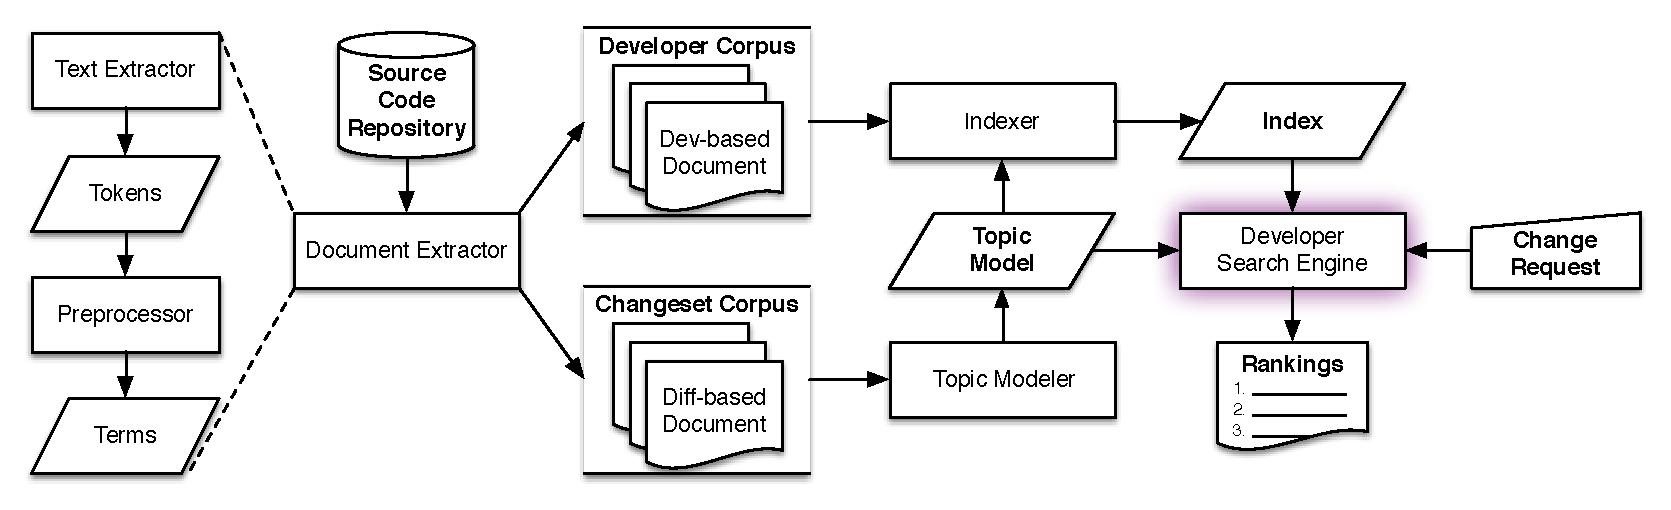
\includegraphics{figures/changeset-triage.pdf}
\caption{Developer identification using
changesets\label{fig:changeset-triage}}
\end{figure}

The changeset topic modeling approach requires two types of document
extraction: and one for the every changeset in the source code history
and a developer profile of the words each individual developer changed
in those changesets. The left side of Figure \ref{fig:changeset-triage}
illustrates the dual-document extraction approach.

The document extraction process for the changesets remains the same as
covered in Section \ref{flt-proposed-approach}.

The right side of Figure \ref{fig:changeset-triage} illustrates the
retrieval process. The key intuition to our approach is that a topic
model such as LDA or LSI can infer any given document's topic
proportions regardless of the documents used to train the model. Hence,
we train a topic model on the changeset corpus, but search for related
developers over the developer corpus. In the search engine, we can use a
dynamic programming to keep \(\theta_{Developers}\) up-to-date as new
changesets are added to the model. That is, upon a update to the model,
new inferences of only the source code documents affected by this
changeset are made. Additionally, we can then query the model as needed
and rank the results of that query against \(\theta_{Developers}\). Note
that we never infer a \(\theta_{Changeset}\) for the changeset documents
on which the model is built.

To leverage the online functionality of the topic models, we can also
intermix the model training and retrieval steps. First, we initialize a
model in online mode. Then, as changes are made, the model is updated
with the new changesets as they are committed. That is, with changesets,
we incrementally update a model and can query it at any moment. This
insight means that we can also evaluate our approach \emph{temporally}.
That is, we we can approximate how the automatic developer
identification would perform throughout the evolution of a project.

\subsubsection{Evaluation}\label{evaluation-1}

\begin{itemize}
\itemsep1pt\parskip0pt\parsep0pt
\item
  DIT using both LSI and LDA
\item
  Datasets?
\item
  We can also do temporal stuff to approximate how the DIT would perform
  throughout the evolution of a project.
\end{itemize}

\section{Combining and Configuring Changset-based Topic
Models}\label{study-config}

\subsection{Motivation}\label{motivation-3}

\subsection{Background}\label{background}

\subsection{Proposal}\label{proposal-2}

\subsubsection{Approach}\label{approach-2}

\begin{figure}[htbp]
\centering
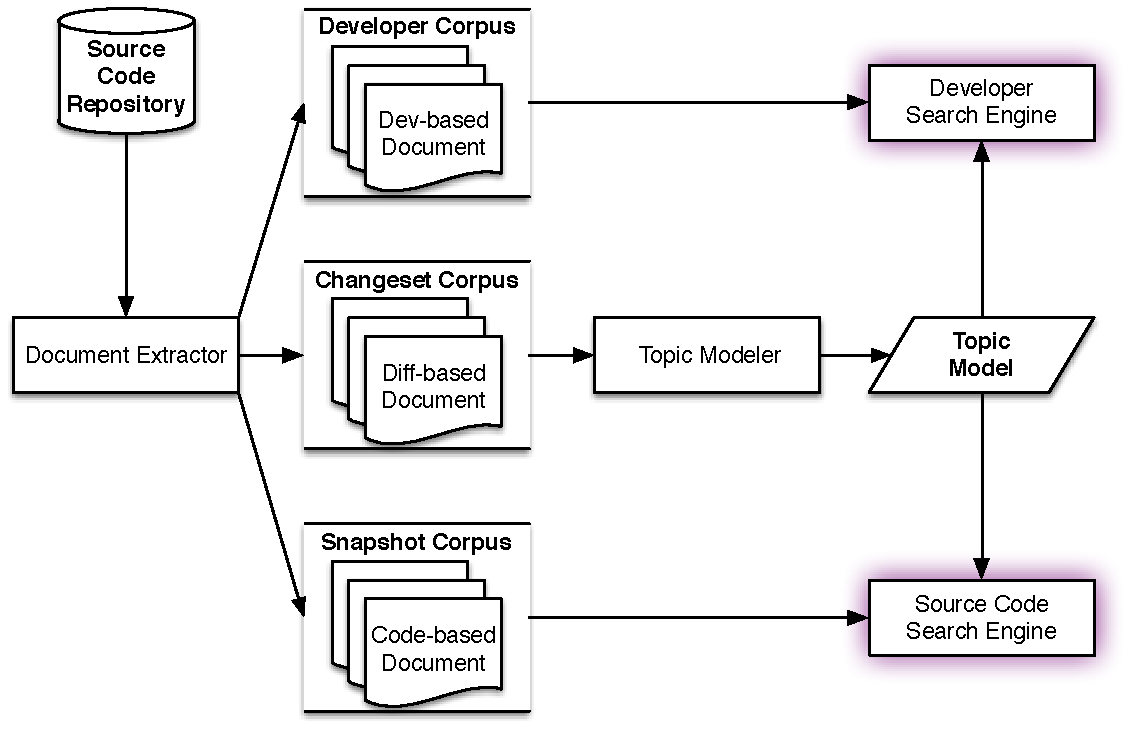
\includegraphics{figures/changeset-combo.pdf}
\caption{Combining changeset-based feature location and developer
identifiation \label{fig:changeset-combo}}
\end{figure}

\subsubsection{Evaluation}\label{evaluation-2}

\chapter{Conclusion}\label{conclusion}

Um
\end{body}

\renewcommand\bibname{References}
\bibliography{proposal}


    \appendix
    \begin{appendices}

\chapter{Projected Schedule}
\begin{subappendices}
Sometime
\end{subappendices}

\end{appendices}


\end{document}
